\section{Data dimensionality reduction and visualization}

After preprocessing, our data was further manipulated in order to reduce its dimensionality.
This allows observation of the data into lower dimensions and gaining insight on how the data is organized, and whether it is linked in meaningful ways~\cite{cunningham2014},~\cite{valletta2017}.
Reducing the dimensionality also allows to plot the data in graphs that are visually meaningful, since after the third dimension, this becomes increasingly difficult.

\subsection{Behavioral data}

Because the goal of the project is to understand the relationship between the DNs of \textit{Drosophila} and its behavior, the behavioral and neural data must be formatted to allow for comparison.
In the case of the behavioral data, which was recorded at \SI{100}{\hertz}, it means downsampling the data to match the \SI{16}{\hertz} of the neural data.
In the downsampled dataset, the distinction between the predicted and manually labeled categorical value for the behavioral classes was merged altogether, with only one label per sample (instead of two, one predicted, one manual).
That label is based on both the predicted and manually labeled values, by considering the most prevalent categorical behavior within the time frame considered for the downsampling.
Indeed, the manual labeling done previously on the initial dataset had proven that the predictions were quite bad: in the original behavioral dataset, there is 22\% of mismatch between the manual labels (67430 mismatches for 302400 total samples), which are summarized in Table~\ref{tab::behavioral_data_count}.

\begin{table}[htbp]
	\sffamily
	\arrayrulecolor{white}
	\arrayrulewidth=1pt
	\renewcommand{\arraystretch}{1.5}
	\rowcolors[\hline]{1}{.!50!White}{}
	\centering
	\begin{tabular}{@{} A|A|B @{}}
		\cellcolor{ForestGreen}\arraycolor{White}\bfseries Behavior prediction &
		\cellcolor{ForestGreen}\arraycolor{White}\bfseries Manual behavior labeling &
		\cellcolor{ForestGreen}\arraycolor{White}\bfseries Count \\   
		\arraycolor{Black}
		Resting & Walking & 13645 \\
		Resting & Anterior grooming & 12745 \\
		Walking & Anterior grooming & 12020 \\
		Walking & Resting & 10641 \\
		Resting & Abdominal pushing & 4156 \\
		Front leg Grooming & anterior grooming & 4143 \\
		Walking & Abdominal pushing & 2806 \\
		Front leg grooming & Walking & 1730 \\
		Antennal grooming & Anterior grooming & 1390 \\
		Walking & Posterior grooming & 1109 \\
		Front leg grooming & Resting & 866 \\
		Resting & Posterior grooming & 835 \\
		Abdominal grooming & Abdominal pushing & 455 \\
		Abdominal grooming & Resting & 164 \\
		Front leg grooming & Posterior grooming & 111 \\
		Antennal grooming & Walking & 108 \\
		Eye grooming & Anterior grooming & 103 \\
		Hind leg grooming & Abdominal pushing & 102 \\
		Abdominal grooming & Walking & 75 \\
		Abdominal grooming & Posterior grooming & 49 \\
		Hind leg grooming & Walking & 32 \\
		Antennal grooming & Posterior grooming & 31 \\
		Antennal grooming & Resting & 22 \\
		Hind leg grooming & Posterior grooming & 16 \\
		Front leg grooming & Abdominal pushing & 12 \\
		Eye grooming & Resting & 9 \\
		Hind leg grooming & Resting & 9 \\
		Eye grooming & Walking & 6 \\
		Antennal grooming & Abdominal pushing & 5 \\
		Eye grooming & Posterior grooming & 4 \\
		Abdominal grooming & Anterior grooming & 0 \\
	\end{tabular}
	\caption{Differences between behavioral predictions and manual labeling.}
	\label{tab::behavioral_data_count}
\end{table}

\vspace{\baselineskip}

This downsampling led to a reduced behavioral dataset comprised of nine categorical values, summarized in Table~\ref{tab::behavioral_data_length}.
Notably, the eye grooming label disappeared (it was only predicted a few times, but not witnessed during the manual labeling), while some new behaviors not manually labeled were introduced, coming from the predicted behaviors.

\begin{table}[htbp]
	\sffamily
	\arrayrulecolor{white}
	\arrayrulewidth=1pt
	\renewcommand{\arraystretch}{1.5}
	\rowcolors[\hline]{1}{.!50!White}{}
	\centering
	\begin{tabular}{@{} A|B @{}}
		\cellcolor{ForestGreen}\arraycolor{White}\bfseries Behavior &
		\cellcolor{ForestGreen}\arraycolor{White}\bfseries Length \\   
		\arraycolor{Black}
		Walking 			& 23228 \\
		Resting 			& 18834 \\
		Anterior grooming 	& 4412 	\\
		Abdominal pushing 	& 1157 	\\
		Front leg grooming 	& 321 	\\
		Posterior grooming 	& 304 	\\
		Antennal grooming 	& 165 	\\
		Abdominal grooming 	& 57 	\\
		Hind leg grooming 	& 2 
	\end{tabular}
	\caption{Categorical values in the reduced behavioral dataset.}
	\label{tab::behavioral_data_length}
\end{table}

\subsection{Kinematic data}

Both the kinematic data and the neural data contain a lot of information.
The kinematic data alone describes 132 temporal variables, at \SI{100}{\hertz} for $\sim\SI{250}{\second}$ over twelve trials.
In order not to fall prey to the curse of dimensionality and sparsity which follows, the kinematic data was projected through a Principal Component Analysis (PCA).
A PCA projects $n$ samples of $p$-dimensional data in an orthogonal, also $p$-dimensional space, the trick being that the destination space, which dimensions are called principal components, are ordered by variance of the data explained and computed so that each successive one explains the most variance possible.
Thus, the higher dimensions of the projected space explain the most variance, while the last explain the least variance.
If the data is entirely uncorrelated, a PCA should explain approximately the same amount of variance per principal component, while a highly correlated dataset will have most of its variance explained by the first principal components.

\vspace{\baselineskip}

Here, the kinematic dataset was separated between the joint angles and the joint positions, and then a PCA was ran on each trial.
Thus, there was a total of 24 PCA.
For the joint positions, the $p$ dimensions of the dataset are the 90 temporal joint position variables, while each temporal point is a sample.
For the joint angles, the $p$ features are the 42 temporal joint angle variables.

\vspace{\baselineskip}

After the PCA, we applied a wavelet transform to analyze the dynamics of the fly's joints.
We used the normalized Morlet wavelet transform from the \verb*|behavelet| package \cite{berman2014}, which analyses the frequency components of the leg segments movements across time.
The Morlet wavelet is composed of a complex exponential multiplied by a Gaussian window, which allows the detection of short oscillations in the time domain.
The Morlet wavelet was applied to the output of the PCA.

\vspace{\baselineskip}

In order to have different visualizations of the dataset, we also applied a t-distributed Stochastic Neighbor Embedding (t-SNE).
Contrary to a PCA, a t-SNE is a non linear method.
It finds mapping of the data points which preserve local neighborhood by first constructing a probability distribution over pairs of similar high-dimensional data points.
Then it defines a similar probability distribution in the low-dimensional map and minimize the Kullback-Leibler (KL) divergence between the two distributions.
The KL divergence is a measure of the difference between the probability distributions.
The t-SNE was applied both directly after the PCAs, and after the wavelet transforms; both for the joint positions and joint angles.
The results are displayed on Figure~\ref{fig::kinematic_data_tsne}.

\begin{figure}[htbp]
	\begin{subfigure}{.49\textwidth}
		\begin{center}
			\includesvg[width=\textwidth]{tsne_joint_pca_s}
			\caption{t-SNE of joint positions from PCA data}
		\end{center}
	\end{subfigure}
	\begin{subfigure}{.49\textwidth}
		\begin{center}
			\includesvg[width=\textwidth]{tsne_joint_wave_s}
			\caption{t-SNE of joint positions from wavelet data}
		\end{center}
	\end{subfigure}
	\begin{subfigure}{.49\textwidth}
		\begin{center}
			\includesvg[width=\textwidth]{tsne_angle_pca_s}
			\caption{t-SNE of joint angles from PCA data}
		\end{center}
	\end{subfigure}
	\begin{subfigure}{.49\textwidth}
		\begin{center}
			\includesvg[width=\textwidth]{tsne_angle_wave_s}
			\caption{t-SNE of joint angles from wavelet data}
		\end{center}
	\end{subfigure}
	\caption{t-SNE plots on the kinematic data after dimensionality reduction.}
	\label{fig::kinematic_data_tsne}
\end{figure}

On Figure~\ref{fig::kinematic_data_tsne}, the data is segregated by behavioral categories.
Unfortunately, it did not produce a meaningful output that would help gain insight on the organization of the kinematic data.

\subsection{Neural data}

\subsubsection{Each neuron a feature, each time point a sample}

We first applied PCA on the neural data with each neuron as a feature and each time point as a sample.
The three first principal components are plotted on Figure~\ref{fig::neural_data_pca1}.

\begin{figure}[htbp]
	\begin{center}
		\begin{subfigure}{\textwidth}
			\begin{center}
				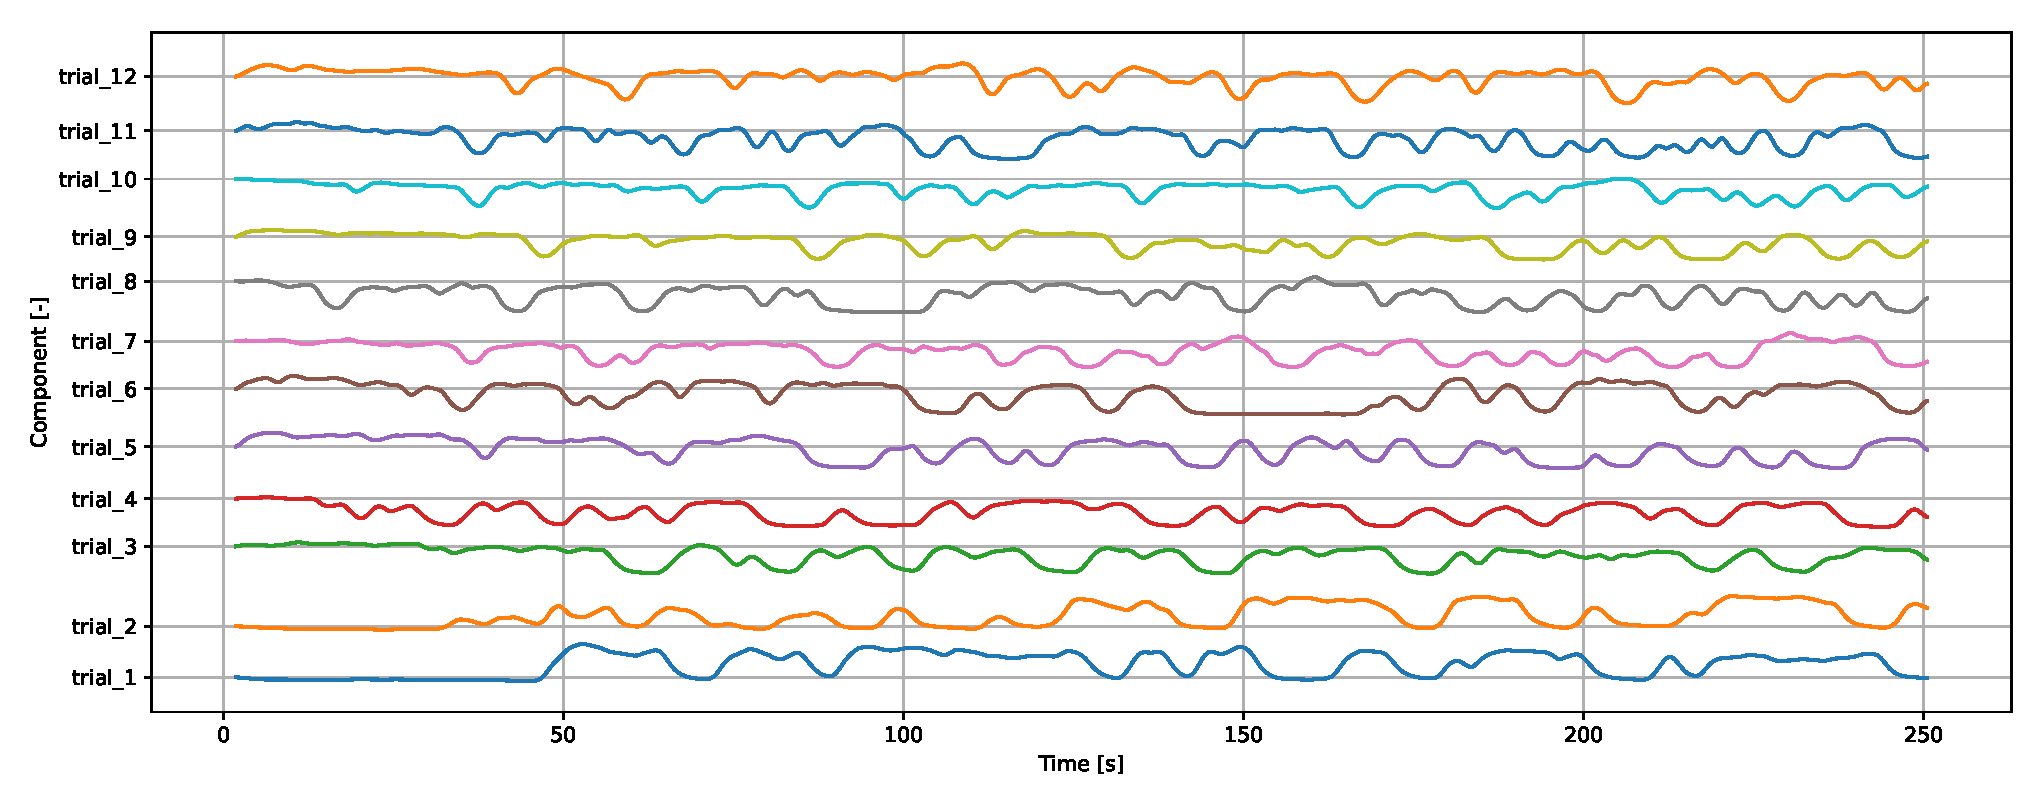
\includegraphics[width=\textwidth]{nd_pca_component_0}
				\caption{Component 0}
			\end{center}
		\end{subfigure}
		\newline
		\begin{subfigure}{\textwidth}
			\begin{center}
				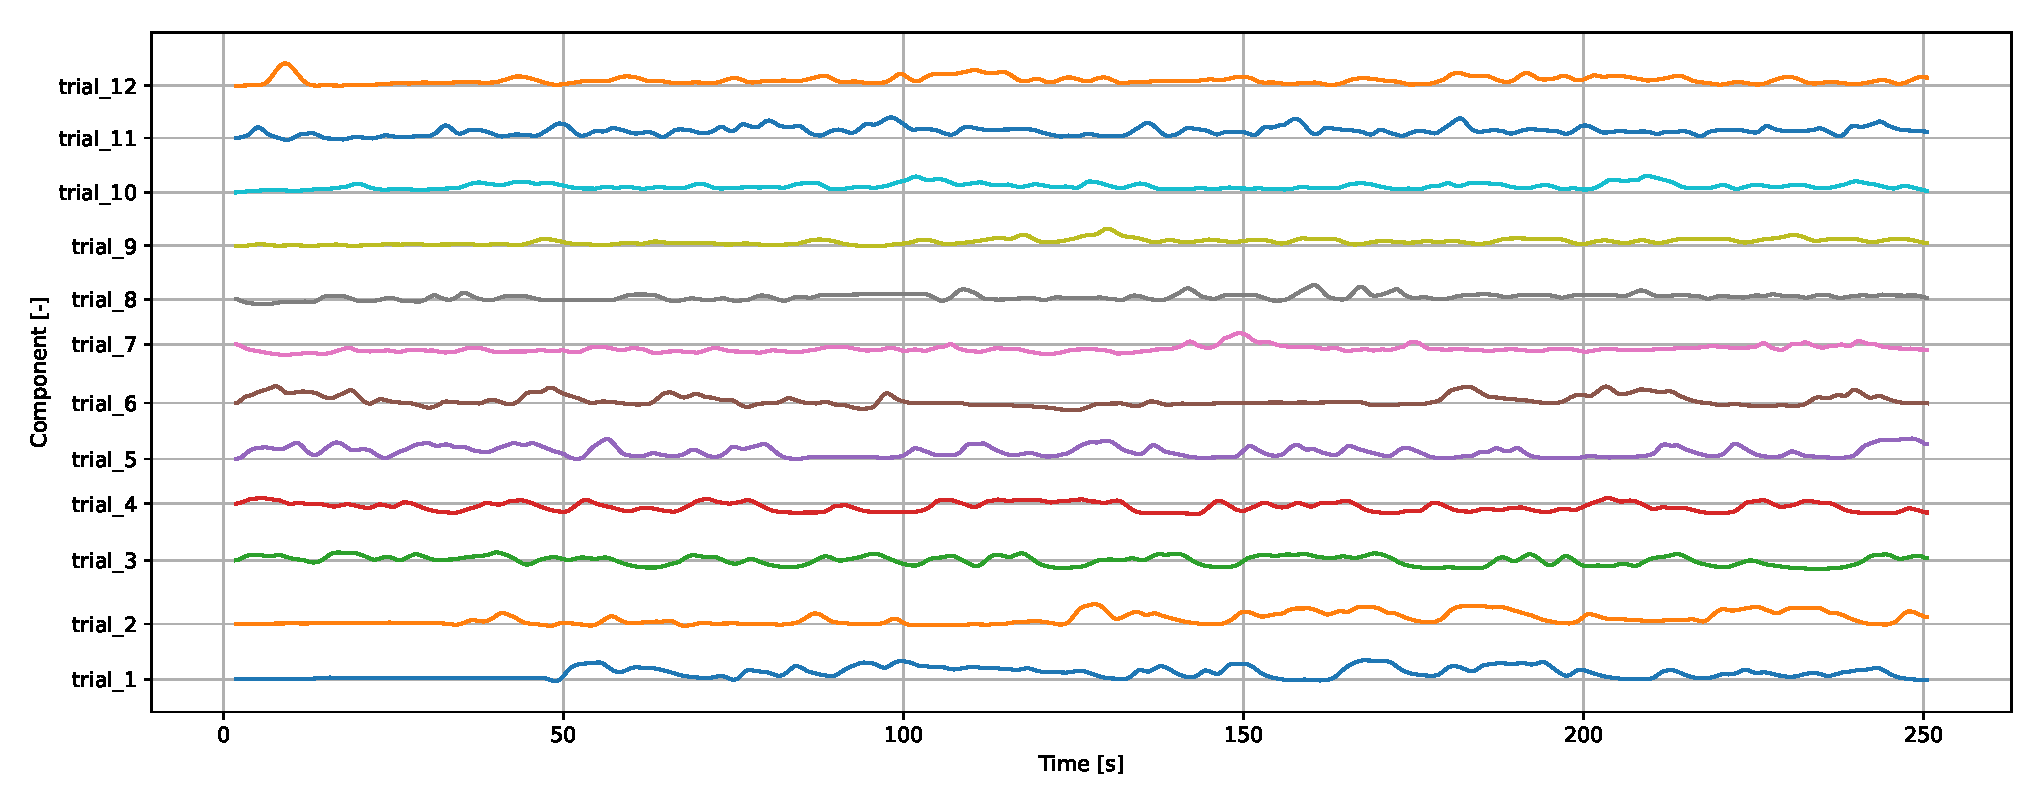
\includegraphics[width=\textwidth]{nd_pca_component_1}
				\caption{Component 1}
			\end{center}
		\end{subfigure}
		\newline
		\begin{subfigure}{\textwidth}
			\begin{center}
				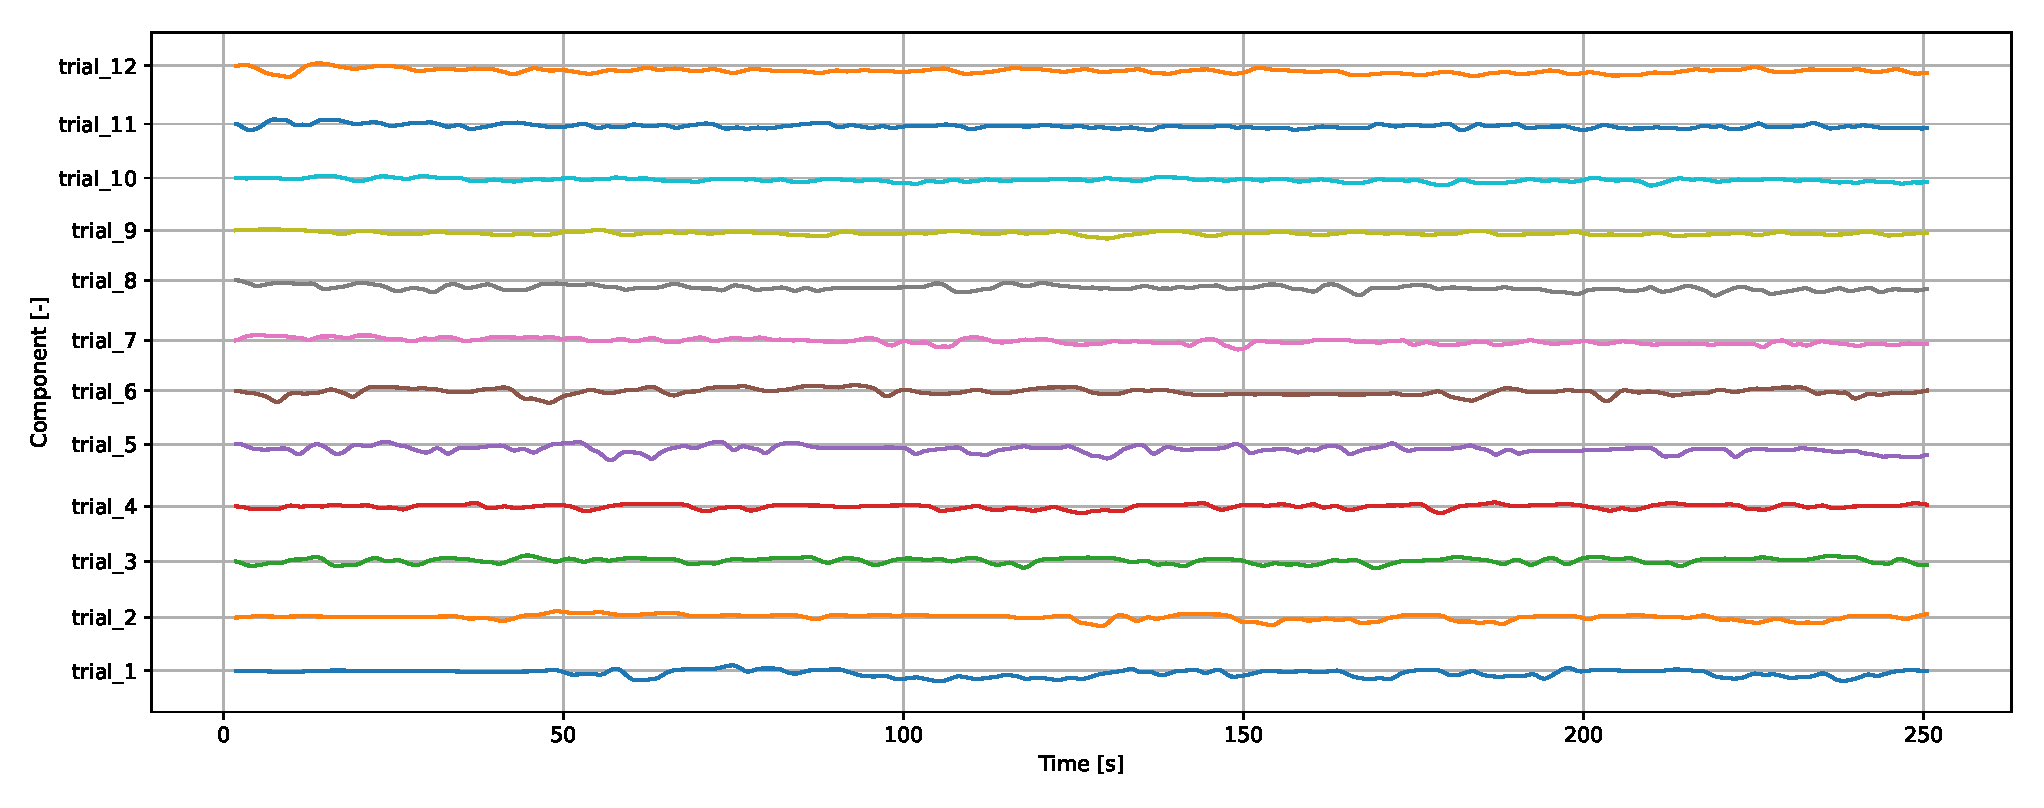
\includegraphics[width=\textwidth]{nd_pca_component_2}
				\caption{Component 2}
			\end{center}
		\end{subfigure}
		\caption{First components of the neural data first PCA (each neuron a feature, each time point a sample).}
		\label{fig::neural_data_pca1}
	\end{center}
\end{figure}

The main observation is that the more we advance in the principal components, the less the signals exhibit variation.
This is due to the fact that PCAs' principal components are specifically constructed to explain the maximum variance in succession.
In this instance, the first 10 components are enough to explain 90\%, as can be seen on Figure~\ref{fig::neural_data_pca1_explained}.
This is quite a low number of components, considering that the initial neural data is composed of 123 dimensions (features).

\begin{figure}[htbp]
	\begin{center}
		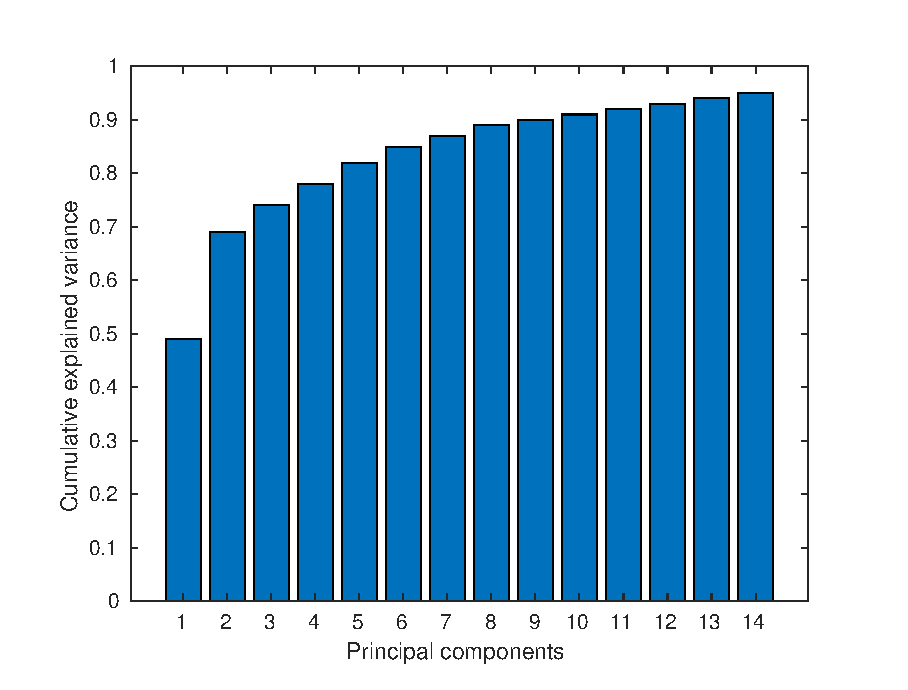
\includegraphics[width=0.6\textwidth]{neural_data_pca1_explained}
		\caption{Cumulative explained variance of the first principal components of the neural data first PCA.}
		\label{fig::neural_data_pca1_explained}
	\end{center}
\end{figure}

The first two principal components explain 69\% of the variance of the neural data.
When plotted in a scatter plot, there are three very obvious clusters (two main at the bottom, one less pronounced on top), as can be seen on Figure~\ref{fig::neural_data_pca1_scatter}.

\begin{figure}[htbp]
	\begin{center}
		\includegraphics[width=0.6\textwidth]{dcsp_2_components_pca}
		\caption{Density-coded scatter plot of the first two components of the neural data first PCA.}
		\label{fig::neural_data_pca1_scatter}
	\end{center}
\end{figure}

That drove us to plot the same data, but this time segregating the samples according to the behavioral categories, as on Figure~\ref{fig::neural_data_pca1_scatter_classes}.

\begin{figure}[htbp]
	\begin{subfigure}{.52\textwidth}
		\begin{center}
			\includesvg[width=\textwidth]{neural_data_pca1_classes}
			\caption{with all the behavioral categories}
		\end{center}
	\end{subfigure}
	\begin{subfigure}{.46\textwidth}
		\begin{center}
			\includesvg[width=\textwidth]{neural_data_pca1_classes_reduced}
			\caption{when regrouping all the grooming categories}
		\end{center}
	\end{subfigure}
	\caption{Behavioral categories segregated scatter plot of the first two components of the neural data first PCA.}
	\label{fig::neural_data_pca1_scatter_classes}
\end{figure}

On Figure~\ref{fig::neural_data_pca1_scatter_classes}, it becomes clear that the two main clusters identified on Figure~\ref{fig::neural_data_pca1_scatter} correspond to actual behavioral categories (respectively resting and walking).
The third cluster however, the one less pronounced on Figure~\ref{fig::neural_data_pca1_scatter}, does not match a specific category.
Rather, it seems that a lot of behaviors can fall in that region of the scatter plot.
When merging all the grooming and pushing behaviors in one unique behavior, it still is not enough to allow for a good bijective mapping:

\begin{itemize}
	\item a point in either bottom clusters allow to identify either walking or resting behaviors,
	\item a point somewhere else on the plot doesn't allow for behavioral discrimination,
	\item and more importantly, choosing a category (any category) does not allow to infer the position of the sample on the scatter plot.
\end{itemize}

However, it still means that some neurons exhibit similar activity when the fly performs either walking or resting.
One benefit of such a redundancy could be a robustness to perturbation when transmitting neural information.

\vspace{\baselineskip}
 
Further manipulation with the application of t-SNE on top of the first PCA lead to the results displayed on Figure~\ref{fig::neural_data_tsne1_scatter}.

\begin{figure}[htbp]
	\begin{center}
		\includegraphics[width=0.6\textwidth]{dcsp_tsne_2_components_pca}
		\caption{Density-coded scatter plot of the t-SNE obtained from the neural data first PCA.}
		\label{fig::neural_data_tsne1_scatter}
	\end{center}
\end{figure}

Unfortunately, it is not a very useful visualization of the data.

\subsubsection{Each neuron as a sample, and each time point as a feature}

Then, we tried to apply the PCA on the neural data again, but the other way round: each neuron as a sample, and each time point as a feature.
Because there are 12 trials, and 4040 time points per trials (so 48480 time points in total), it is necessary for that PCA to reduce the number of time points.
Indeed, viewing the data with this features / samples perspective would not make sense if there were 48480 dimensions and only 123 samples, that would make it a very sparse dataset.
Thus, the data was first averaged over each trial, so that there is only 12 samples left.
The scatter plot of that second PCA is displayed on Figure~\ref{fig::neural_data_pca2_scatter}.

\begin{figure}[htbp]
	\begin{center}
		\includesvg[width=0.6\textwidth]{neural_data_pca2_scatter}
		\caption{Density-coded scatter plot of the neural data second PCA.}
		\label{fig::neural_data_pca2_scatter}
	\end{center}
\end{figure}

Afterwards, another t-SNE was applied to try and see if that leads to interesting results.
They are displayed on Figure~\ref{fig::neural_data_tsne2_scatter}.

\begin{figure}[htbp]
	\begin{subfigure}{.49\textwidth}
		\begin{center}
			\includesvg[width=\textwidth]{neural_data_tsne2_scatter_density}
			\caption{density-coded visualization}
		\end{center}
	\end{subfigure}
	\begin{subfigure}{.49\textwidth}
		\begin{center}
			\includesvg[width=\textwidth]{neural_data_tsne2_scatter_kmeans}
			\caption{k-means clustering}
		\end{center}
	\end{subfigure}
	\caption{Scatter plot of the t-SNE obtained with the neural data second PCA.}
	\label{fig::neural_data_tsne2_scatter}
\end{figure}

We observe three clusters, which means that we have essentially clustered neurons that exhibit correlation in their temporal behavior.

\newpage
